% !TeX root = ../index.tex
\chapter{Week 1}
\graphicspath{{1-week-1/images/}}

\section{Exercise 1}

\url{https://intweb.bucks.ac.uk/~21606555/oos/1-week-1/ex1.php}
\captionsetup{type=figure}\captionof{figure}{ex1.php}
\subfile{pyg/src/1-week-1/ex1}

\begin{figure}[H]
  \caption{Output of exercise 1}
  \centering
  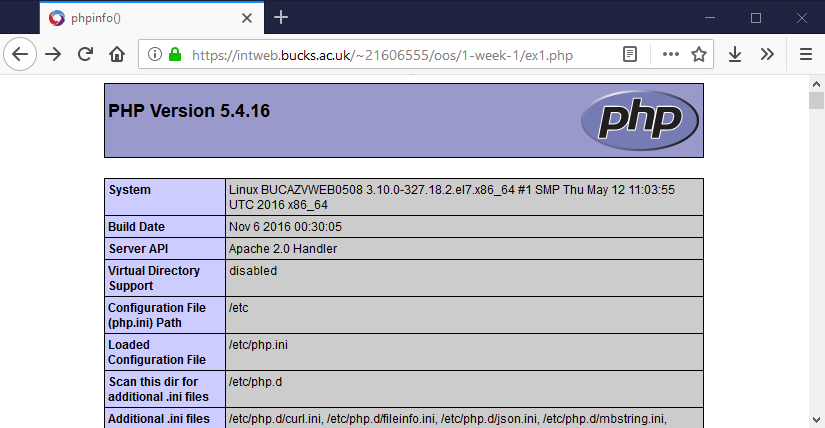
\includegraphics[width=\textwidth]{ex1}
\end{figure}

\clearpage
\section{Exercise 2}

\url{https://intweb.bucks.ac.uk/~21606555/oos/1-week-1/ex2.php}
\captionsetup{type=figure}\captionof{figure}{ex2.php}
\subfile{pyg/src/1-week-1/ex2}

\begin{figure}[H]
  \caption{Output of exercise 2}
  \centering
  \includegraphics[width=\textwidth]{ex2}
\end{figure}

\section{Exercise 3}

\url{https://intweb.bucks.ac.uk/~21606555/oos/1-week-1/ex3.php}
\captionsetup{type=figure}\captionof{figure}{ex3.php}
\subfile{pyg/src/1-week-1/ex3}

\begin{figure}[H]
  \caption{Output of exercise 3}
  \centering
  \includegraphics[width=\textwidth]{ex3}
\end{figure}

\section{Exercise 4}

The last argument of \texttt{gmddate()\texttt} allows you to provide a specific date to format. This argument is optional and will use the current date and time if it is not provided.\\

\url{https://intweb.bucks.ac.uk/~21606555/oos/1-week-1/ex4.php}
\captionsetup{type=figure}\captionof{figure}{ex4.php}
\subfile{pyg/src/1-week-1/ex4}

\begin{figure}[H]
  \caption{Output of exercise 4}
  \centering
  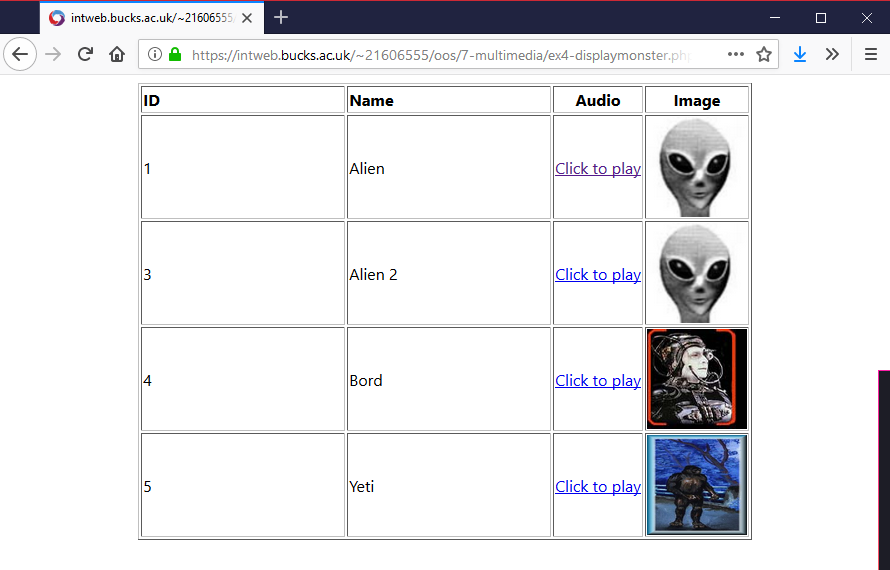
\includegraphics[width=\textwidth]{ex4}
\end{figure}

\clearpage
\section{Exercise 5}

\url{https://intweb.bucks.ac.uk/~21606555/oos/1-week-1/ex5.php}
\captionsetup{type=figure}\captionof{figure}{ex5.php}
\subfile{pyg/src/1-week-1/ex5}

\begin{figure}[H]
  \caption{Output of exercise 5}
  \centering
  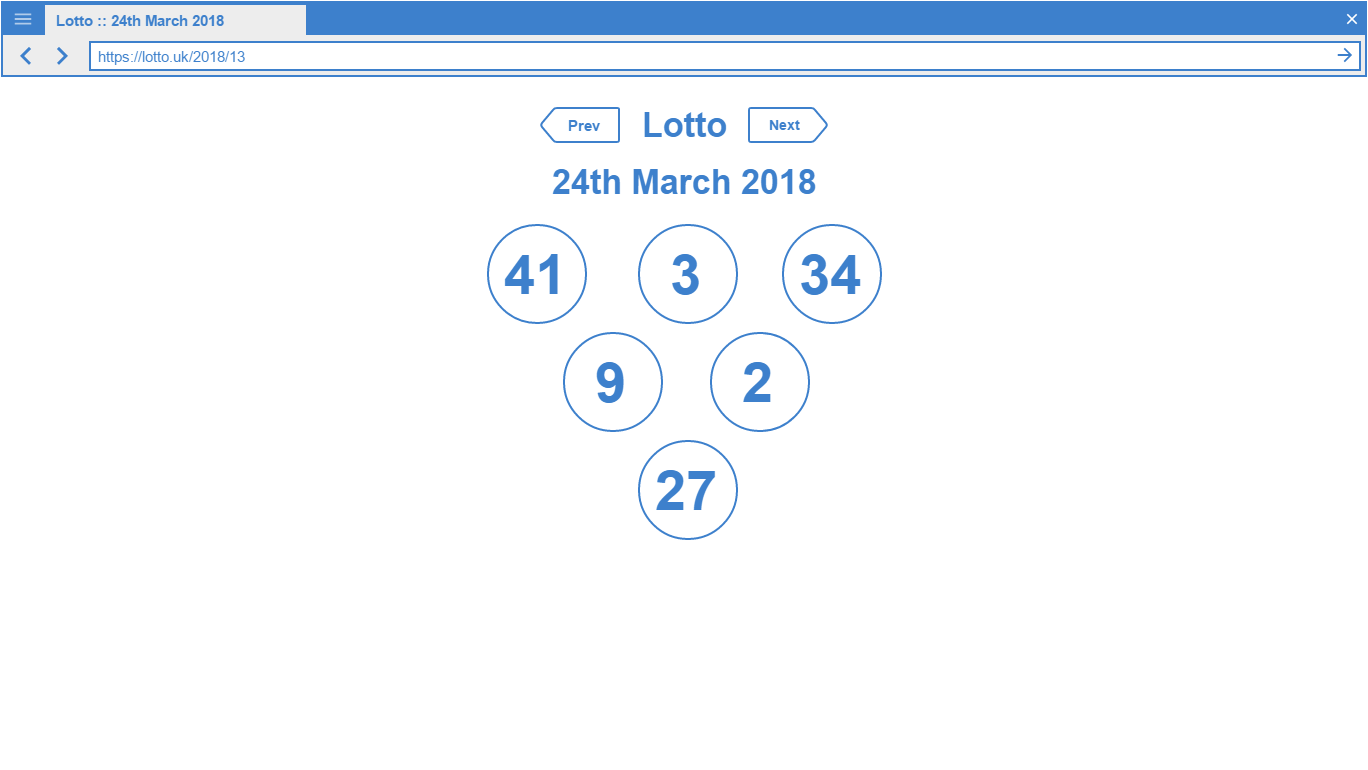
\includegraphics[width=\textwidth]{ex5}
\end{figure}

\section{Exercise 6}

\url{https://intweb.bucks.ac.uk/~21606555/oos/1-week-1/ex6.php}
\captionsetup{type=figure}\captionof{figure}{ex6.php}
\subfile{pyg/src/1-week-1/ex6}

\begin{figure}[H]
  \caption{Output of exercise 6}
  \centering
  
\includegraphics[width=\textwidth]{ex6}
\end{figure}

\section{Exercise 7}

\url{https://intweb.bucks.ac.uk/~21606555/oos/1-week-1/ex7.php}
\captionsetup{type=figure}\captionof{figure}{ex7.php}
\subfile{pyg/src/1-week-1/ex7}

\begin{figure}[H]
  \caption{Output of exercise 7}
  \centering
  \includegraphics[width=\textwidth]{ex7}
\end{figure}
